%        File: homework2.tex
%     Created: Fri Jan 23 01:00 PM 2015 P
% Last Change: Fri Jan 23 01:00 PM 2015 P
%
\documentclass[11pt]{article}
\usepackage{geometry}
\usepackage{graphicx}
\usepackage{enumerate}
\geometry{letterpaper}
\usepackage[parfill]{parskip}
\title{Math 360 Homework 2}
\author{Alex Schneider}
\begin{document}
\maketitle
\section*{Handout}
\subsection*{Problem 1}
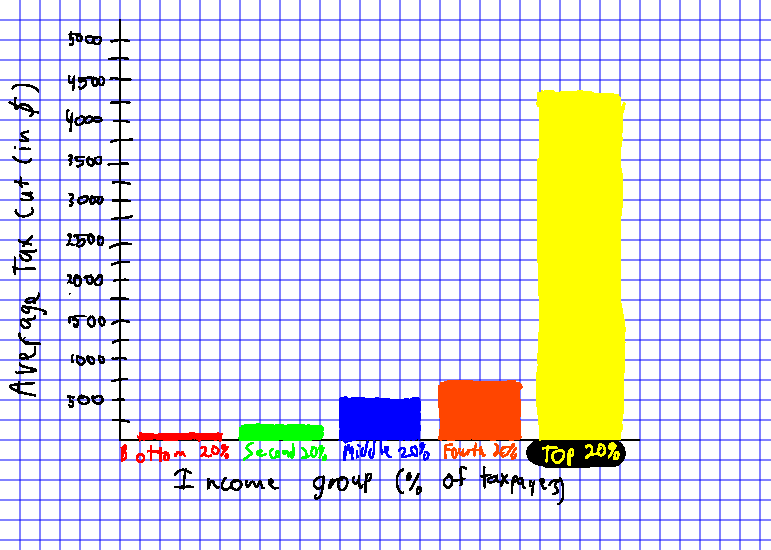
\includegraphics{homework2_handout_problem1_bargraph}

\subsection*{Problem 2}
Given the three values of \$0, \$289, and \$1211, and being asked to determine which
ones are the mean, median, and mode of the tax cuts, I would probably come up
with the following conclusions:

\subsubsection*{Mode}
\[M_0 = \$0\]
Due to the nature of money, nice round numbers out of these types of tax cuts
rarely happen. Therefore, the only round number that we can reasonably expect
is no tax cuts at all, and even if there a relatively few number of people who
received that, it is still a more likely outcome. 

Secondly, it is unlikely for the median or mean to be 0, unless tax cuts are
negative, which they don't appear too be. 

\subsubsection*{Median}
\[M_d = \$289\]
We established that the median cannot be 0. We also know that the median has to 
be somewhere between the second 20\% (\$212) and fourth 20\% (\$951). This
prevents \$1211 from being the median, so we're left with \$289 as our only
option.

\subsubsection*{Mean}
\[\overline{X} = \$1211\]
By process of elimination, we're left with \$1211 as the only candidate for the
mean. In addition, we know that there are a large amount of outliers in the top
20\% which can bring the mean up pretty drastically.

\subsection*{Problem 3}
If I could draw a new bar graph reflecting the new information, I would reach
the limits of information provided by a linear scale. The outliers are so high
that the bar graph would either need to be incredibly large or there would need
to be a misleading break in the middle of the graph. If that were the case, I
would probably go for a graph on a \textit{log} scale to give a more faithful
representation to the data, at the cost of misleading those unfamiliar with
logarithms into thinking the difference is much less than it is. 

\section*{Section 1.3}
\subsection*{Problem 1}
\subsubsection*{a.}
\begin{tabular}{r|l} % chktex 44
    Stem & Leaf \\
    \hline % chktex 44
    0 & 011112235677 \\
    1 & 235579 \\
    2 & 468 \\
    3 & 11257 \\
    4 & 1469 \\
    5 & 5 \\
    6 & 16 \\
    7 & 9 \\
    8 & 0099 \\
    11 & 0 \\
    12 & 7 \\
    13 & 7
\end{tabular}

\subsubsection*{b.}
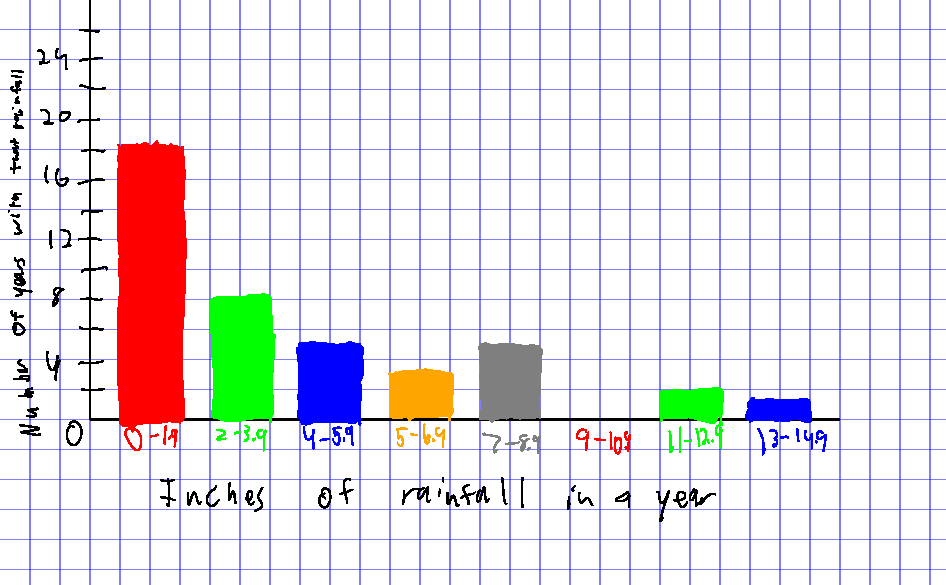
\includegraphics{homework2_section13_problem1b_histogram}

\subsubsection*{c.}
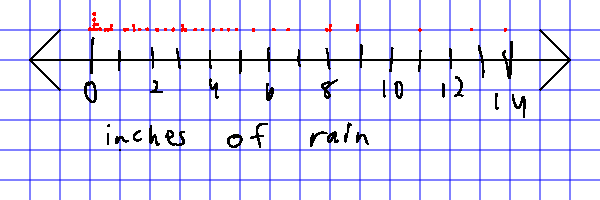
\includegraphics{homework2_section13_problem1c_dotplot}

\subsubsection*{d.}
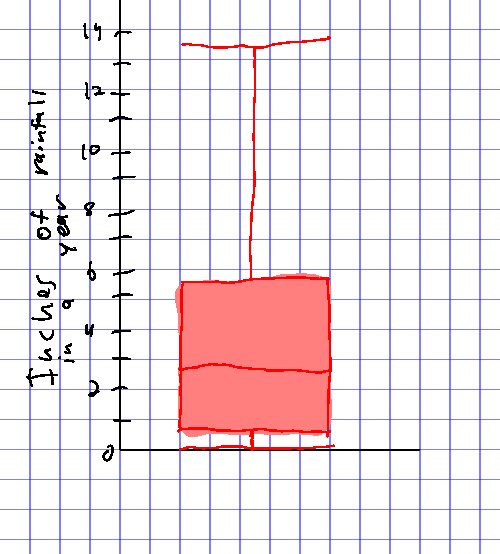
\includegraphics{homework2_section13_problem1d_boxandwhisker}

Yes, the box plot appears to show significant outliers at the top of the
rainfall measurements. 

\subsection*{Problem 2}
\subsubsection*{b.}
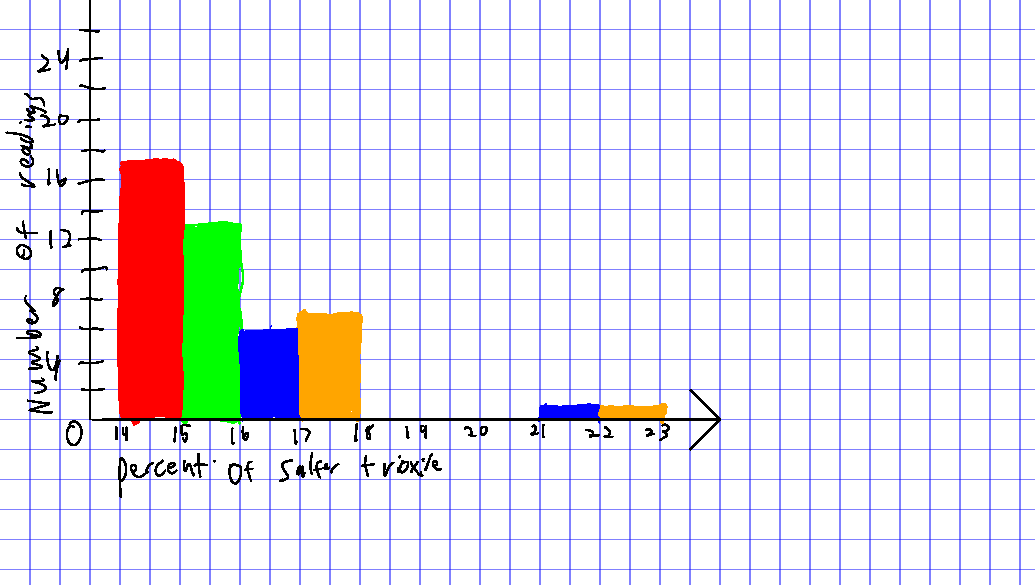
\includegraphics{homework2_section13_problem2b_histogram}

\subsubsection*{c.}
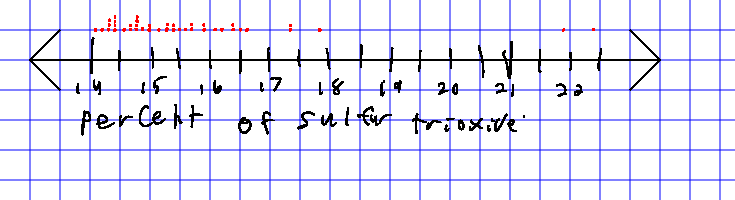
\includegraphics{homework2_section13_problem2c_dotplot}

\subsection*{Problem 6}
\subsubsection*{a.}
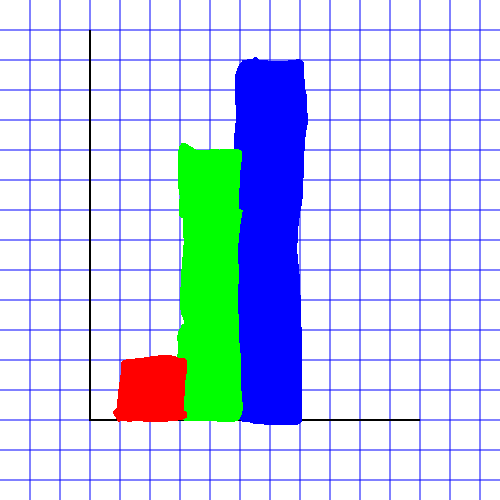
\includegraphics{homework2_section13_problem6a_histogram}

\subsubsection*{b.}
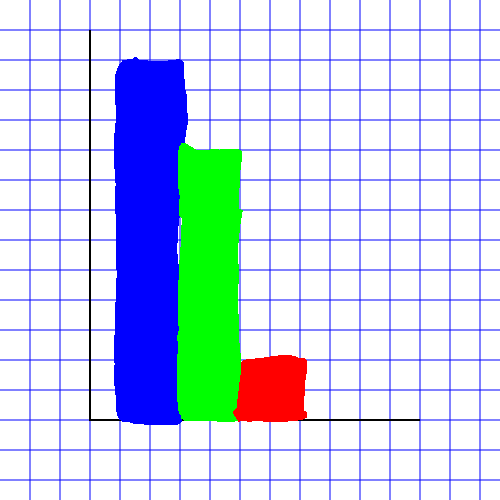
\includegraphics{homework2_section13_problem6b_histogram}

\subsubsection*{c.}
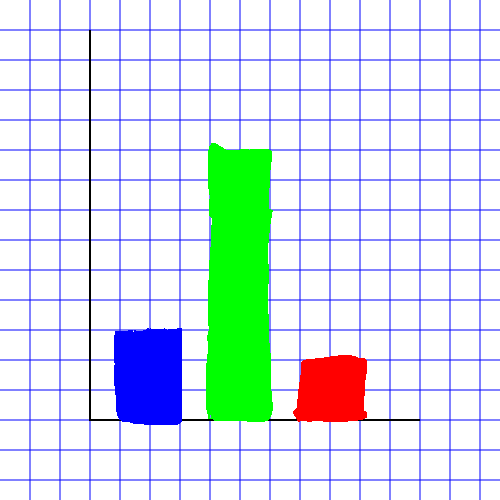
\includegraphics{homework2_section13_problem6c_histogram}

\subsection*{Problem 7}
\subsubsection*{a.}
The percentage of women with blood pressures above 130mm is likely closest to
25\% of the sample represented by the histogram. 

\subsubsection*{b.}
There are more women in the 130--135mm interval.

\subsection*{Problem 12}
A boxplot cannot determine \textit{ii}. The mean.

This is because the box plot is entirely constructed based off of quartile
information. Although a mean can be approximated by a boxplot, there isn't
enough information to state it exactly. 

\subsection*{Problem 16}
\begin{enumerate}
    \item \textit{c}
    \item \textit{b}
    \item \textit{d}
    \item \textit{a}
\end{enumerate}

\subsection*{Problem 18}
\begin{enumerate}[i]
    \item \textit{b}
    \item \textit{d}
    \item \textit{a}
    \item \textit{c}
\end{enumerate}

\section*{Section 2.1}
\subsection*{Problem 1}
The probability that the bearing will not fail during the first month of use is
$1.00 - 0.12$ or $0.88$. 

\subsection*{Problem 2}
\subsubsection*{a.}
The sample space is as follows:
\[ \textit{S} = \left\{ 1, 1, 1, 2, 2, 3 \right\} \]

\subsubsection*{b.}
$P(odd number)$ is as follows:
\[ P(odd number) = P(1) + P(3) \] 
\[ P(odd number) = \frac{3}{6} + \frac{1}{6} \]
\[ P(odd number) = \frac{4}{6} = \frac{2}{3} \]
\[ P(odd number) \approx 0.\overline{6} \]

\subsubsection*{c.}
No, the sample space would remain the same. The sample space is just a listing
of the possibilities and gives no information as to the probability of a
possibility occurring. 

\subsubsection*{d.}
Yes, the value of $P(odd\;number)$ would increase slightly. It wouldn't increase
by a full $\frac{1}{6}$ because it would be taking away from the probability of
rolling a $1$. 

\subsection*{Problem 3}
\subsubsection*{a.}
The sample space is as follows:
\[ \textit{S} = \left\{ 
    \begin{array}{c}
        \left( T, T, T, T \right),
        \left( T, T, T, F \right),
        \left( T, T, F, T \right),
        \left( T, T, F, F \right),\\
        \left( T, F, T, T \right),
        \left( T, F, T, F \right),
        \left( T, F, F, T \right),
        \left( T, F, F, F \right),\\
        \left( F, T, T, T \right),
        \left( F, T, T, F \right),
        \left( F, T, F, T \right),
        \left( F, T, F, F \right),\\
        \left( F, F, T, T \right),
        \left( F, F, T, F \right),
        \left( F, F, F, T \right),
        \left( F, F, F, F \right)
    \end{array}
\right\} \]

\subsubsection*{b.}
The probability that all answers are the same is as follows:
\[ P(same) = P\left( \left( T, T, T, T \right) \right) + 
             P\left( \left( F, F, F, F \right) \right)
\]
\[ P(same) = \frac{1}{16} + \frac{1}{16} \]
\[ P(same) = \frac{1}{8} \]
\[ P(same) = 0.125 \]

\subsubsection*{c.}
The probability that exactly one answer is ``True'' is as follows:
\[ P(one\;true) = P((T, F, F, F)) +
                 P((F, T, F, F)) +
                 P((F, F, T, F)) +
                 P((F, F, F, T))
\]
\[ P(one\;true) = \frac{1}{16} + \frac{1}{16} + \frac{1}{16} + \frac{1}{16} \]
\[ P(one\;true) = \frac{1}{4} \]
\[ P(one\;true) = 0.25 \]

\subsubsection*{d.}
The probability that at most one answer will be true is as follows:
\[ P(up\;to\;one\;true) = P(one\;true) + P((F, F, F, F)) \]
\[ P(up\;to\;one\;true) = \frac{1}{4} + \frac{1}{16} \] 
\[ P(up\;to\;one\;true) = \frac{5}{16} \] 
\[ P(up\;to\;one\;true) = 0.3125 \]

\subsection*{Problem 4}
\subsubsection*{a.}
\[ S = \left\{ 
    \begin{array}{c}
        \left( R, R, R \right),
        \left( R, R, Y \right),
        \left( R, R, G \right),
        \left( R, Y, R \right),
        \left( R, Y, Y \right),
        \left( R, Y, G \right),
        \left( R, G, R \right),
        \left( R, G, Y \right),
        \left( R, G, G \right), \\
        \left( Y, R, R \right),
        \left( Y, R, Y \right),
        \left( Y, R, G \right),
        \left( Y, Y, R \right),
        \left( Y, Y, Y \right),
        \left( Y, Y, G \right),
        \left( Y, G, R \right),
        \left( Y, G, Y \right),
        \left( Y, G, G \right), \\
        \left( G, R, R \right),
        \left( G, R, Y \right),
        \left( G, R, G \right),
        \left( G, Y, R \right),
        \left( G, Y, Y \right),
        \left( G, Y, G \right),
        \left( G, G, R \right),
        \left( G, G, Y \right),
        \left( G, G, G \right)
    \end{array}
\right\} \]

\subsubsection*{b.}
\[ A = \left\{ 
    \begin{array}{c}
        \left( R, R, R \right),
        \left( Y, Y, Y \right),
        \left( G, G, G \right)
    \end{array}
\right\} \]

\subsubsection*{c.}
\[ B = \left\{ 
    \begin{array}{c}
        \left( R, Y, G \right),
        \left( R, G, Y \right),
        \left( Y, R, G \right),
        \left( Y, G, R \right),
        \left( G, R, Y \right),
        \left( G, Y, R \right)
    \end{array}
\right\} \]

\subsubsection*{d.}
\[ C = \left\{ 
    \begin{array}{c}
        \left( R, G, G \right),
        \left( Y, G, G \right), 
        \left( G, R, G \right),
        \left( G, Y, G \right),
        \left( G, G, R \right),
        \left( G, G, Y \right),
        \left( G, G, G \right)
    \end{array}
\right\} \]

\subsubsection*{e.}
\[ A \cap C = \left\{ 
    \begin{array}{c}
        \left( G, G, G \right)
    \end{array}
\right\} \]

\subsubsection*{f.}
\[ A \cup B = \left\{ 
    \begin{array}{c}
        \left( R, R, R \right),
        \left( R, Y, G \right),
        \left( R, G, Y \right),
        \left( Y, R, G \right),
        \left( Y, Y, Y \right), \\
        \left( Y, G, R \right),
        \left( G, R, Y \right),
        \left( G, Y, R \right),
        \left( G, G, G \right)
    \end{array}
\right\} \]

\subsubsection*{g.}

\[ A \cap C^c = \left\{ 
    \begin{array}{c}
        \left( R, R, R \right),
        \left( Y, Y, Y \right)
    \end{array}
\right\} \]

\subsubsection*{h.}
\[ A^c \cap C = \left\{ 
    \begin{array}{c}
        \left( R, G, G \right),
        \left( Y, G, G \right), 
        \left( G, R, G \right),
        \left( G, Y, G \right),
        \left( G, G, R \right),
        \left( G, G, Y \right)
    \end{array}
\right\} \]

\subsubsection*{i.}
\textit{A} and \textit{C} share one outcomes, that is if all lights are green
(outcome $(G, G, G)$). Therefore, they are not mutually exclusive events. 

\subsubsection*{j.}
\textit{B} and \textit{C} share no outcomes. Therefore, they are mutually
exclusive events. 

\subsection*{Problem 7}
\subsubsection*{a.}
The probability of a TV set being located in the living room or the den is as
follows:

\[ P(living\;or\;den) = P(living) + P(den) \]
\[ P(living\;or\;den) = 0.26 + 0.22 \]
\[ P(living\;or\;den) = 0.48 \]

\subsubsection*{b.}
The probability of a TV set not being located in the bedroom is as follows:

\[ P(not\;bedroom) = 1 - P(bedroom) \]
\[ P(not\;bedroom) = 1 - 0.01 \]
\[ P(not\;bedroom) = 0.99 \]

\subsection*{Problem 8}
\subsubsection*{a.}
The probability of a customer being a good risk is as follows:

\[ P(good\;risk) = 70\% \]
\[ P(good\;risk) = 0.7 \]

\subsubsection*{b.}
The probability of a customer not being a poor risk is as follows:

\[ P(not\;poor\;risk) = 1 - P(poor\;risk) \]
\[ P(not\;poor\;risk) = 1 - 10\% \]
\[ P(not\;poor\;risk) = 1 - 0.1 \]
\[ P(not\;poor\;risk) = 0.9 \]

\subsection*{Problem 9}
\subsubsection*{a.}
The probability of a randomly chosen part having a flaw is as follows:
\[ P(flaw) = P(major) + P(minor) \]
\[ P(flaw) = 0.05 + 0.15 \]
\[ P(flaw) = 0.2 \]

\subsubsection*{b.}
The probability of a randomly chosen part having no major flaw is as follows:
\[ P(no\;major) = 1 - P(major) \]
\[ P(no\;major) = 1 - 0.05 \]
\[ P(no\;major) = 0.95 \]

\subsection*{Problem 12}
\subsubsection*{a.}
The probability that a computer contains both a virus and a worm is as follows:
\[ P(V\&W) = P(V) + P(W) - P(V\cup W) \]
\[ P(V\&W) = 0.15 + 0.05 - 0.17 \]
\[ P(V\&W) = 0.03 \]

\subsubsection*{b.}
The probability that a computer contains neither a virus nor a worm is as
follows:
\[ P(healthy) = 1 - P(V \cup W) \]
\[ P(healthy) = 1 - 0.17 \]
\[ P(healthy) = 0.83 \]

\subsubsection*{c.}
The probability that a computer contains a virus, but not a worm is as follows:
\[ P(V\&\;not\;W) = P(V \cup W) - P(W) \]
\[ P(V\&\;not\;W) = 0.17 - 0.05 \]
\[ P(V\&\;not\;W) = 0.12 \]

\subsection*{Problem 13}
\subsubsection*{a.}
The probability that a student has taken statistics, chemistry, or both is as
follows:

\[ P(S\;or\;C) = P(S) + P(C) - P(S\cap C)\]
\[ P(S\;or\;C) = 0.4 + 0.3 - 0.2 \]
\[ P(S\;or\;C) = 0.5 \]

\subsubsection*{b.}
The probability that a student has taken neither stats nor chemistry is as
follows:

\[ P(neither) = 1 - P(S\;or\;C) \]
\[ P(neither) = 1 - 0.5 \]
\[ P(neither) = 0.5 \]

\subsubsection*{c.}
The probability that a student has taken statistics, but not chemistry is as
follows:

\[ P(S\;not\;C) = P(S) - P(S\cap C) \]
\[ P(S\;not\;C) = 0.4 - 0.2 \]
\[ P(S\;not\;C) = 0.2 \]

\subsection*{Problem 17}
The probability of a system functioning is as follows:

\[ P(functioning) = P(A) + P(B) - P(A\;or\;B) \]
\[ P(functioning) = 0.98 + 0.95 - 0.99 \]
\[ P(functioning) = 0.94 \]

\subsection*{Problem 18}
\subsubsection*{a.}
The probability that a randomly chosen blood donor is type O is as follows:

\[ P(type\;O) = 1 - \left( P(AB) + P(A) + P(B) \right) \]
\[ P(type\;O) = 1 - \left( 0.05 + 0.35 + 0.10 \right) \]
\[ P(type\;O) = 0.5 \]

\subsubsection*{b.}
The probability that a randomly chosen blood donor may donate to a type A
recipient is as follows:

\[ P(can\;donate) = P(A) + P(O) \]
\[ P(can\;donate) = 0.35 + 0.5 \]
\[ P(can\;donate) = 0.85 \]

\subsection*{Problem 19}
\begin{enumerate}[a.]
    \item True --- neither A nor B have any outcomes, in common or otherwise.
    \item True --- neither A nor B have any outcomes in common.
    \item False --- though this can be the case for \textit{a} and
        \textit{b}, it isn't necessarily the case, for example, suppose A = all
        positive odd numbers less than 10, and B = all positive odd numbers less
        than 10. 
    \item True --- This can only be the case if there is no overlap between A and
        B. 
\end{enumerate}

\end{document}


